\documentclass{report}
\usepackage[utf8]{inputenc}
\usepackage[textheight=650pt]{geometry}
\usepackage{graphicx}
\usepackage{float}

\begin{document}
\newcommand{\arrow}{-\textgreater}

\title{Zusammenfassung Technikgeschichte}
\author{aqulu}
\maketitle
\tableofcontents
\newpage

\chapter{Einführung}

\section{Was ist Technik?}
Griech. ``technikos``: Handwerk, Kunst, Kunstfertigkeit\\
\begin{itemize}
	\item Das ``Gemachte`` (Artefakte, aus dem Latein: mit Kunst gemacht)
	\item Deren Herstellung
	\item Deren Verwendung. 
\end{itemize}~\\
Phil. Frage (was ist heute der Fall?): 
\begin{description}
	\item[Technikdeterminismus] Technik dominiert den Menschen
	\item[Konstruktivismus] Technik folgt den menschlichen Bedürfnissen
\end{description}

\subsection{Warum Technik?}
\begin{itemize}
	\item Keine biologische Spezialisierung des Menschen -\textgreater~künstliche Spezialisierung durch Technik
	\item Neue Bedürfnisse -\textgreater~Entwicklung neuer Technik (mit Erlaubnis)
	\item Entlastung durch Energie (bessere Lebensqualität durch geringeren Energieverbrauch bei Arbeit)
\end{itemize}

\newpage
%--------------NEW PAGE -----------------------------

\section{Technikgeschichte}
befasst sich mit den Fragen:
\begin{itemize}
	\item Wieso wurde ein technisches Angebot gemacht?
	\item Von wem wurde ein technisches Angebot gemacht?
	\item Für wen wurde ein technisches Angebot gemacht?
	\item Auswirkungen des neuen technischen Angebots auf Gesellschaft, Wirtschaft und Politik
\end{itemize}

\subsection{Eisenbahn-Beispiel}
\textbf{Wieso und von wem erfunden?}
\begin{itemize}
	\item Günstiger Transport von Material in Bergwerken
	\item in Grossbritannien ``erfunden``
	\item Grosse Nachfrage nach Kohle, da Holz nicht mehr als Energielieferant zur Verfügung (in GB)
\end{itemize}~\\
\textbf{Auswirkungen}
\begin{itemize}
	\item Günstiger Transport von Mensch \& Massengütern über grosse Strecken
	\item Grossstädte möglich (transport von Gütern in die Stadt, Transport von Abfall aus der Stadt)
	\item Zeit wird zentraler Aspekt im Leben
\end{itemize}

\newpage
%--------------NEW PAGE -----------------------------

\chapter{Geschichte bis zur industriellen Revolution}
\section{Erste Hochkulturen}
\begin{description}
	\item[vor 10'000 Jahren] Ende der Eiszeit -\textgreater~ Neolithische Revolution
	\item[2000 v. Chr.] Erste Hochkulturen in Ägypten und Zweistromland
		\begin{itemize}
			\item Bewässerungssysteeme
				\begin{itemize}
					\item Bildung Herren / Kneche Gesellschaft
					\item Trennung Waffen und Werkzeug
					\item Herrschaftsbildung durch die Schrift
				\end{itemize}
			\item Herstellung von Glas \& Bronze
			\item Wagenrad, Töpferscheibe, Pflug
		\end{itemize}
	\item[1500 v. Chr.] Eisenberarbeitung -\textgreater~ Übergang zur Antike
\end{description}

\newpage
%--------------NEW PAGE -----------------------------

\section{Antike}
\begin{itemize}
	\item 8.Jahrhundert v. Chr. bis 5. Jahrhundert n. Chr.
	\item Metallverarbeitung (dominant aber Holz \& Stein)
	\item Energie = menschl. Muskelkraft (Sklaven)
	\item Werkzeuge wirken mit Hebelkraft
	\item Techniken übernommen / teilw. leicht verbessert
	\item Nahrungsüberschuss -\textgreater~ imperiale Expansion
\end{itemize}

\subsection{Griechenland}
\subsubsection{Archimedes von Syrakus \rm{\textit{287 - 217 v. Chr.}}}
Erster Techniker der Weltgeschichte
Verbindet Technik und Wissenschaft, Geometrie und Maschinenkonstruktion\\\\
\textbf{Erfindungen:}
\begin{itemize}
	\item Flaschenzug
	\item Archimedische Schraube
	\item Hebelgesetz
	\item Nutzung expandierender Wasserdampf
\end{itemize}

\subsection{Rom}
Weltreich zwischen Spanien und dem heutigen Irak und zwischen England und Nord-Afrika\\\\
\textbf{Techniken:}
\begin{itemize}
	\item Wasserleitungen
	\item Monumentalbauten
	\item Strassen
\end{itemize}

\newpage
%--------------NEW PAGE -----------------------------

\section{Mittelalter}
\begin{itemize}
	\item von 1000 bis 1500
		\begin{itemize}
			\item 1000 bis 1350 (Pest): Zeit des Aufbruchs und der Erneuerung
			\item 1350 bis 1450: Zeit der Stagnation
		\end{itemize}
	\item Pflug, Kummet und Mühle in der Landwirtschafts
		\begin{itemize}
			\item Pflug von Ochsen und Pferden gezogen -\textgreater~Verdoppelung Erträge
			\item Zweiteilung Bauernschaft
			\item Wassermühlen und Windmühlen
			\item Hammerschmiede zur Eisenbearbeitung
		\end{itemize}
	\item Zunahme Gewerbe -\textgreater~Vergrösserung Städte
	\item Verbot technischer Entwicklungen, die Arbeitsplätze vernichten könnten\\(weniger Arbeitsplätze = Hunger)
\end{itemize}

\subsection{Technische Entwicklung}
Gemächlicher technischer Fortschritt durch Übernahmen und Weiterentwicklungen – selten Eigenentwicklungen
\begin{itemize}
	\item Einführung Spinnrad -\textgreater~Verdoppelung Erträge
	\item Entwicklung Trittwebstuhl (in Flandern)
		\begin{itemize}
			\item dreifache Produktionssteigerung 
			\item Weber wird ein Beruf
		\end{itemize}
	\item ca. 1290: Erfindung Uhr (einzige europ. Erfindung)
		\begin{itemize}
			\item Zeitökonomie entsteht
			\item mechanisch-lineare Zeitvorstellung
		\end{itemize}
	\item ab 1400: Taschenuhren (Federnbremse und Schnecke)
		\begin{itemize}
			\item ab 1600: Minuten werden beachtet
		\end{itemize}
	\item ca. 1300: Entwicklung Brille
\end{itemize}

\newpage
%--------------NEW PAGE -----------------------------

\subsection{Zeit der Zünfte}
\subsubsection{Zünfte \rm{(= städtische Berufsgenossenschaft)}}
\begin{itemize}
	\item Monopolisierung gewerblichen Wissens und gewerblicher Tätigkeit (um die Nahrungssicherheit zu bekommen)
	\item Zünfte beginnen ihre Bereiche selber zu regeln
		\begin{itemize}
			\item Werden zu politischer und militärischen Organisation\\
			-\textgreater~Bruch Herrschaft der Fürsten\\
			-\textgreater~Ende des Feudalismus
		\end{itemize}
	\item ``Stadtluft macht frei! ``\\
		\textit{In der Stadt wohnende Unfreie können nach 1 Jahr und 1 Tag in Freiheit nicht mehr vom Dienstherrn zurückgefordert werden}
	\item Lohnverhältnis Meister (Zünfter) - Arbeiter
	\item Organisation der Berufsbildung 
		\begin{itemize}
			\item Lehrzeit, Prüfung, Wanderschaft – Meisterprüfung
		\end{itemize}
\end{itemize}

\section{Renaissance}
\begin{itemize}
	\item 1436: Erfindung Buchdruck\\
	-\textgreater~1500: 27'000 Werke mit Auflage von 20 Mio. erschienen
	\item Entdeckungsreisen
		\begin{itemize}
			\item Kolumbus (Amerika)
			\item da Gama (Indien)
		\end{itemize}
	\item Perspektive in Gemälden
	\item Herstellung Beton
\end{itemize}

\subsubsection{Leonardo da Vinci \rm{\textit{1452 - 1519}}}
\begin{itemize}
	\item Künstler, Architekt
	\item Musiker, Wissenschaftler
	\item Mediziner, Geologe
	\item Zeichner und Maler
\end{itemize}

\newpage
%--------------NEW PAGE -----------------------------

\section{Reformation}
ca. von 1517 bis 1661\\
\begin{itemize}
	\item Arbeit wird zentrales moralisches Element des Lebens
	\item Arbeit als Anerkennung und Geschenk Gottes angesehen
	\item Bibel = einzige göttl. Wahrheit; alle sollten sie lesen können
	\item Reichtum kein Laster\\
	-\textgreater~Erlaubnis Zinsen und Bankgeschäfte für Christen
	\item Keine Dogmen\\
	-\textgreater~mehr Forschungen werden toleriert
	\item bis 1648: grosse Religionskriege in Europa
\end{itemize}

\section{Absolutismus}
ab 1661
\begin{itemize}
	\item Anti-freiheitliche Welle -\textgreater~absolutistische Monarchien
	\item Keine Anwendung von neuen Erfindungen
	\item Domination Merkantilismus (= Wirtschaft mit starken staatlichen Eingriffen)
		\begin{itemize}
			\item Handwerk
			\item Verlagwesen
			\item Manufakturen
		\end{itemize}
	\item Wissenschaftl. Fortschritte in Grossbritannien\\
	-\textgreater~ werden dort zuerst wirtschaftlich nützlich angewendet
\end{itemize}

\chapter{Industrielle Revolution}
\section{Ursachen und Ablauf}
\subsection{Geistige Voraussetzungen}
\subsubsection{Die Aufklärung}
\begin{itemize}
	\item Betrachtaet Vernuft als Prüfstein der Wahrheit\\
		\arrow Was nicht rational begründet werden kann wird als Vorurteil oder Aberglaube abgelehnt
	\item Mensch als vernünftiges Wesen kann Vernunft als Richtschnur für Leben anwenden\\
		\arrow Mensch ist mit Rechten auszustatten
	\item Skeptisch, rationalistisch, optimistisch
	\item ``Cognito ergo sum`` - Ich denke, also bin ich
\end{itemize}

\subsubsection{John Locke}
Begründer der Staatstheorie:\\
Menschen schlossen Gesellschaftsvertrag, um Staat zu bilden.

Mensch \textless \arrow Staat haben gegenseitig Pflichten und Rechte (Freiheitsrecht, Recht auf Leben, Eigentumsgarantie...)

Widerstandsrecht gegenüber Herrschern, die Pflichten nicht nachkommen\\\\
Empirismus:
\begin{itemize}
	\item Ursprung jeder Erkenntnis liegt in der Erfahrung
	\item Wissen entsteht aus der Sinneswahrnehmung
	\item Durch logische Auswertung können Erkenntnisse über Gegenstände gewonnen werden, die der direkten Sinneswahrnehmung entzogen sind
\end{itemize}

\subsubsection{Aufklärung und Naturwissenschaften}
\begin{itemize}
	\item Grundlagen bereits seit 17. Jahrhundert gelegt (Mathematik und Physik)
	\item Geisteshaltung der Aufklärung positive Auswirkungen auf Naturwissenschaften (v.a. Elektrizitätslehre, Wellentheorie des Lichtes, Chemie, Zoologie)
	\item Genauere Messinstrumente  ebenfalls positive Auswirkungen
	\item Mathematisch formulierte Naturgesetze erstmals für praktische Bedürfnisse angewendet
\end{itemize}

\newpage
\subsection{Physiokratismus und klassische Nationalökonomie}
\subsubsection{Physokratismus}
Lehnte Merkantilismus ab - war der Überzeugung, dass nicht Handelsbilanz sondern Urproduktion (Landwirtschafts und Bergbau) zu besserem Volkswohlstand führt

\arrow Anstösse zur Agrar-Revolution

\subsubsection{Klassische Nationalökonomie}
1776 - Adam Smiths Volkswohlfahrt:
\begin{itemize}
	\item Wirtschaft folgt einfachen Grenzen
	\item Wenn jeder für sich schaut, geht es allen besser\\
		\arrow Freie Marktwirtschaft und keine staatlichen Eingriffe in Wirtschaft
	\item Arbeitsteilung führt zu grösserer Produktivität
\end{itemize}

\subsection{Bevölkerungswachstum}
Bevölkerungswachstum Faktor 1.5 (120 Mio zu 190 Mio) im 18. Jahrhundert\\
Verdoppelung im 19. Jahrhundert\\
Ursache: tiefere Säuglingssteblichkeit\\\\
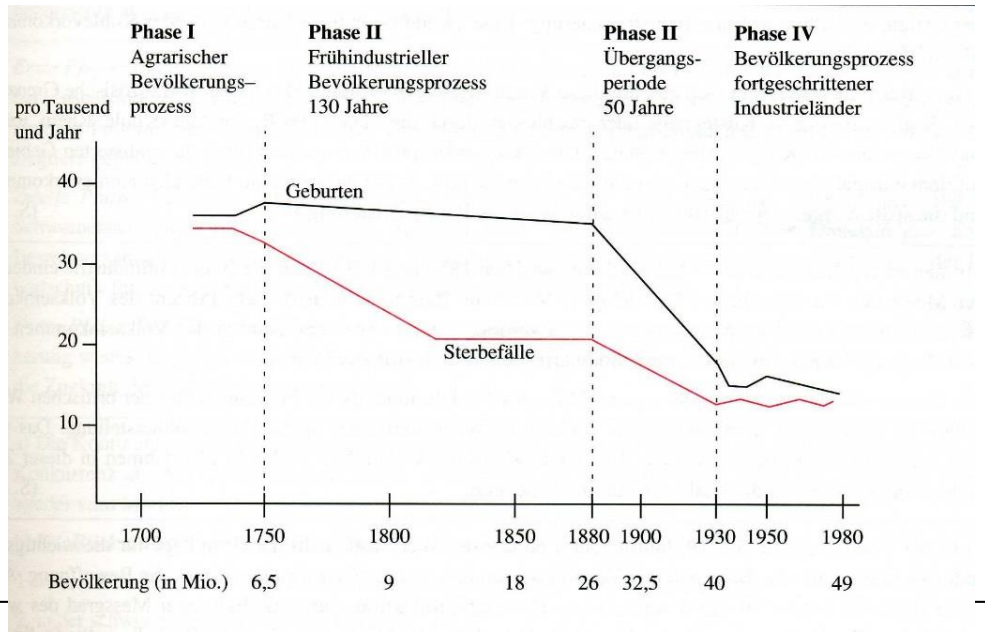
\includegraphics[width=\textwidth]{images/geburtenrate.png}
\newpage

\subsection{Agrar Revolution}
Änderungen in Landwirtschaft führt zu besserer Gesundheit (z.B. durch erhöhten Fleischkonsum in der Schweiz)
\begin{itemize}
	\item Trockenlegung Sumpfgebiete (Bsp.: Linthebene mit Linthkanal)
	\item Ende Dreifelder-Wirtschaft, Einführung Fruchtwechsel-Wirtschaft
	\item Aufteilung der Allmen unter den Bauern
	\item Jauchegruben
	\item Einführung Sommer-Stallfütterung\\
		\arrow 20\% mehr Futterertrag
	\item Einführung Blattfrüchte Klee, Kartoffel und Zuckerrübe
		\arrow Boden wurde auf natürliche Weise mit Stickstoff gedüngt
	\item Mechanisierung durch verbesserte Pflüge, Eggen, Mähmaschinen und Heuwender
	\item ab 1850: Einsatz Kunstdünger (Stickstoff / Phosphate) (Vorher Import Chilesalpeter)
	\item Züchtung Pflanzen und Tiere (nach Darwin und Mendel)
	\item Rationalisierung Viehhaltung\\
		\arrow Schwein wird vom Weidetier zum Stalltier
	\item Abgabe von Kraftfutter
\end{itemize}

\subsection{Wissenschaftliche Veränderungen}
Wissenschaftliche Entdeckungen wurden erst umgesetzt, wenn ein Bedarf für ihren Einsatz und das Kapital vorhanden war
\subsubsection{Bsp. Textilindustrie}
\begin{figure}[H]
	\centering
	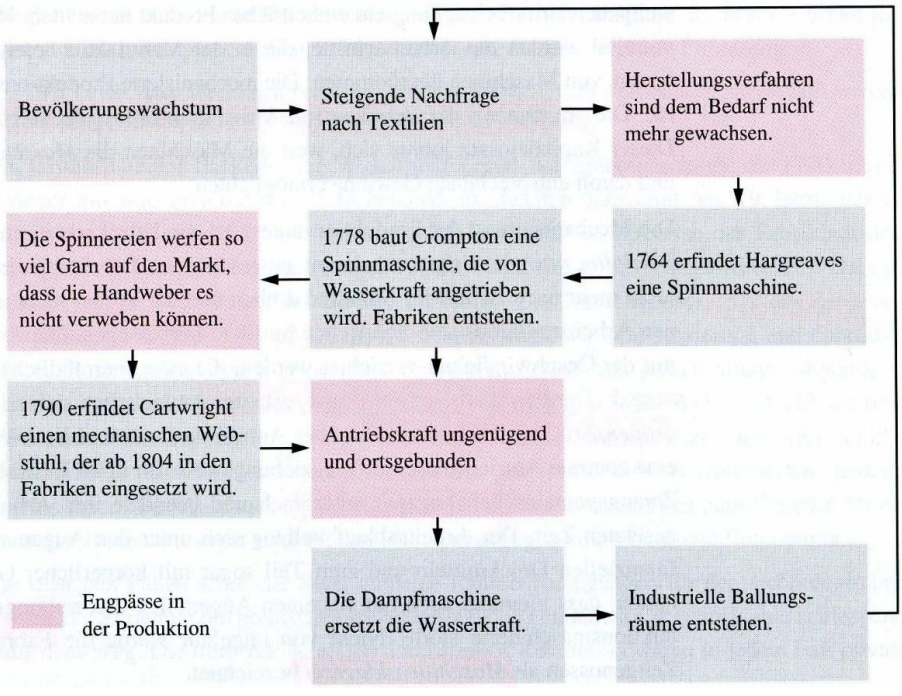
\includegraphics[width=0.75\textwidth]{images/erfindungen-textilindustrie.png}
\end{figure}
\newpage

\subsection{Kapital}
Kapitalbedarf ist wegen Erstausrüstung Fabrik / laufenden Erneuerungen und vermehrte Aufwendungen von Rohstoffen, Löhnen und Energie sind seit der Industriellen Revolution grösser geworden

\subsubsection{Herkunft Kapital}
Spekuklationen um 
\begin{itemize}
	\item Von der wegen der Agrar-Revolution prosperierenden Landwirtschaft
	\item Gewinne aus dem Fernhandel, speziell des Kolonialhandels
	\item Individuelle Ersparnisse des Unternehmers und seiner Verwandtschaft
\end{itemize}
\arrow Sobald der Industrialisierungsprozess in Gang gekommen war, erzeugte dieser das nun benötigte Kapital selber

\subsubsection{Neue Einstellung zur Arbeit}
\begin{itemize}
	\item Vorkapitalistisches Ideal des ``gerechten Preises`` wird durch Gewinnmaximierung ersetzt
	\item Durch freien Arbeitsmarkt (speziell in GB) konnte ländlicher Bevölkerungsüberschuss in Fabrikstädte strömen
	\item Wirtschaftlicher Freiraum wurde (speziell in GB) grösser 
		\arrow Wichtige Entwicklungen:
		\begin{itemize}
			\item Eigentumsgarantie
			\item Das Unterhaus (vom Bügertum dominiert) reduzierte Steuer- und Abgabenbelastung 
			\item Sukzessive Aufhebung der Zunftordnung
		\end{itemize}
	\item Puritaner (englische Reformierte) sahen in materiellen Reichtum Zeichen der Gnade Gottes\\
	Erste industrialisierte Gebiete Europas mehrheitlich von Protestanten bewohnt

\end{itemize}

\subsection{Technische Entwicklung}
\begin{description}
	\item[1764] Baumwollspinnmaschine (J. Hargreaves)
	\item[1769] Mit Wasserkraft betriebene Spinnmaschine (R. Arkwright)
	\item[1784] Mech. Webstuhl (E. Cartwright)
	\item[1785] Mit Dampfkraft angetriebene Baumwollspinnerei
	\item[1807] Dampfschiff
	\item[1830] Eisenbahnlinie Manchester - Liverpool
	\item[1866] Dynamo Starkstrom (Siemens)
	\item[1885] Einsatz von Benzinmotoren in Fahrzeugen (Daimler / Benz)
\end{description}

\newpage

\section{Industrialisierung in Grossbritannien}
\subsection{Voraussetzungen}
\begin{description}
	\item[Geographische Lage] Insel und schiffbare Flüsse \arrow~Grösste Handelsflotte, Navy schützt Insel\\
	\arrow Weltweiter Zugang zu Rohstoffen und Absatzmärkten; keine Binnenzölle

	\item[Religionspolitik] Drei Kirchen leben friedlich miteinander (Puritaner in der Mehrheit)

	\item[Konstitutionelle Monariche] Seit 1689 entschieded Parlament Gesetze und Steuern;	König darf keine Armee unterhalten

	\item[Wirtschaftlich tätiger Adel]

	\item[Konzentration Landwirtschaft] Kleinbauern wurden zu Landarbeitern; Grosse Höfe rationalisierten und produzierten für Städte\\
	\arrow Landarbeiter verloren Arbeit, Abwanderung in Städte

	\item[Ausbau Wasserwege und Strassen] Kein Punkt mehr als 100km von Meer entfernt

	\item[Entwaldung] Grosser Bedarf an Holu (Schiffbau, Eisenverhüttung)\\
	\arrow Gasgewinn aus Steinkohle; Koks als veredelte Kohle (Eisenverhüttung)

	\item[Kohleknappheit] (danach) Abpumpen des Grundwassers
\end{description}

\subsection{Ablauf}
Industrielle Revolution in GB in strakem Zusammenhang mit Baumwollindustrie:\\
Um 1700 England führend in Wollstoffherstellung und Baumwollgewerbe in Anfängen\\\\
Wolle-Importverbot zum Schutz grosser Schafzüchter \arrow~Textilhersteller in Kolonialhäfen wichen auf Baumwollverarbeitung aus\\\\
Nach 7 jährigem Krieg: GB zwang Indien zum Import britischer Baumwollstoffe \arrow~Zerstörung indischer Baumwollindustrie\\
Förderung Baumwollindustrie in Nord-Amerikanischen Kolonien\\\\
Günstige Herstellung durch Sklaven \arrow~Tausch von Baumwollprodukten gegen weitere Sklaven\\\\
Arbeitsprozess dauert lange (Spinnen) \arrow~Erfindung \& Entwicklung Spinnmaschine, Spinnereien\\
\arrow~Industrielle Umstellung der Textilindustrie\\\\
Durch Dampfmaschine konnte Textilindustrie von Flüssen (vorher als Antrieb benötigt) überallhin verlegt werden 

\section{Industrialisierung Europa}
zwischen 1815 und 1830 erschwerte konservative Politik Industrialisierung; Durch liberale Bewerbungen Beschleunigung in vielen Ländern ab 1830 (v.a. FR und BE)\\
Später auch DE und USA (Bürgerkrieg 1861 - 1865)\\
\arrow~ Dominanz GB schwindet langsam; DE und USA als aufstrebende Industrienationen\\\\
Weltwirtschaft ab 1870\\
\arrow~wirtschaftliche Zusammenarbeit stand Politik im Weg; Erster Weltkrieg

\newpage

\chapter{Zweite Industrielle Revolution}
zwischen 1870 und 1880: viele Erfidnungen in Physik und Chemie

\subsubsection{Eisen- und Stahlindustrie}
Günstigere Herstellung durch bessere Verfahren (Bessemerbirne, Martin-Siemens- \& Thomas-Verfahren)\\
\arrow~massiver Ausbau Eisenbahnlinien (diverse Beispiele)

\subsubsection{Elektrotechnische Industrie}
Gleichstromgenerator (1866), Dynamo und Wechselstromgeneratoren (1878) von Siemens\\
Glühlampe (1879) von Edison

\subsubsection{Chemische Industrie}
\begin{itemize}
	\item Anilin- und Teerfarben
	\item Medikamaente
	\item Kali- und Stickstoffdünger
	\item Metallgewinnung durch Elektrolyse
	\item Schwefelsäure
\end{itemize}

\subsubsection{Motorenindustrie \& Verkehrswesen}
Lokomotive (1824) von Stephenson \arrow~ Eisenbahnbau in GB und Europa\\
Billiger Stahl ab 1870 \arrow~massiver Eisenbahnbau\\
Benzinmotor (1883 Patent; 1885 erster Motor) von Benz\\
Dieselmotor (1893)\\\\
Atlantiküberquerung:\par
1860 - 24 Tage mit Schraubendampfer\par
1910 - 8 Tage mit Turbinendampfer
\newpage

\section{Soziales}
Situation der Arbeiterschaft rückt in Vordergrund und stellt Bisheriges in Frage:
\subsection{Arbeitsbedingungen}
\subsubsection{Materielle}
\begin{itemize}
	\item Feuchte, dreckige, gefährliche Arbeitsplätze
	\item Lange Arbeitstage (16h / 6d)
	\item Keine Ferien / Weiterbildung / Freizeit
	\item Bestrafung für Verspätung und Fehler
	\item Schlechter Lohn (teilw. Frauen und Kinderarbeit, da günstiger)
\end{itemize}
\arrow~ Aufstände (Fabrikbrand von Uster 1832; Zerstörungen von Maschinen; Todesstrafe in GB für Maschinenstürmer)

\subsubsection{Rechtliche}
\begin{itemize}
	\item Keine unbefristeten Arbeitsverträge
	\item Einseitige Verpflichtung (Arbeiter \arrow~Arbeitgeber)
	\item Keine Unfall- / Kranken- / Alters- / Arbeitslosenversicherung
	\item Mietskasernen und Fabrikläden führten zu stärkerer Kettung der MA an Unternehmen
\end{itemize}

\subsubsection{Frauen- und Kinderarbeit}
Frauen erledigten schlechtere Arbeiten und erhielten weniger Lohn; Konnten nicht Vorgesetzte von Männern sein; teilw. Doppel / Dreifachbelastung\\
Gebaren teilw. in Fabrik; für möglichst schnelle Rückkehr: Ruhigstellung Kind mit Schnaps\\
Kinder arbeiteten sobald möglich; da Schulpflicht meist in der Nacht

\subsection{Wohnsituation}
\begin{itemize}
	\item Wohnungen werden Spekulationsgut
	\item Wegen den Windverhältnissen in Europa soziale Aufteilung der Städte
	\item Quartiere werden umgebaut um Revolten zu verhindern (Boulevard in Paris)
\end{itemize}

\subsection{Entwicklung}
Technik hilft zur Verbesserung Situation:\\
Konzentrierte, ausgebildete, motivierte Arbeiter nötig für Maschinen\par
\arrow~ Weiterbildung; Weniger Arbeitszeit; Lohnerhöhung; \par Hobbys und Ablenkungen werden gefördert\\\\
Geld und Freizeit führt zu mehr Alkoholismus und Prostitution

\section{Lösung des sozialen Probleme}
\begin{tabular}{l | p{6cm} | p{8cm}}
\textbf{Wer?} & \textbf{Weiso?} & \textbf{Wie?} \\\hline
Arbeiter & Selbsthilfe & Parteien, Gewerkschaften, Streiks, Arbeitervereine \\\hline
Unternehmer & Soziale Gesinnung; Angst vor Aufständen & Schulen, Wohnungen, Krankenhäuser\\\hline
Staat & Sozialer Friede, Angst vor Aufständen, Allgemeine Wehrpflicht & Sozialgesetze, Koalitionsrecht, Senkung Zölle \\\hline
``Kirchen`` & Nächstenliebe, Säkularisierung & Heilsarmee, Gaststätte; Hilfswerke, Heime \\\hline
Philosophen & Bessere Welt & Neue Philosophien; Sozialismus
\end{tabular}

\subsection{Genossenschaftstheorie \rm{\textit{Robert Owen (1771 - 1858)}}}
\begin{itemize}
	\item Unternehmen gehört Arbeitern (erhalten produzierten Mehrwert)\\
	\arrow~Verhältnis zur Arbeit ändert sich
	\item Demokratischere Wirtschaft.
	\item 1848 Idee genossenschaftlichstaatlicher ``Nationalwerkstätte`` in FR
	\item Genossenschaften können günstiger produzieren, privaten Unternehmen werden langfristig durch Konkurrenz untergehen
``Friedlicher`` Weg in den Sozialismus
\end{itemize}

\subsection{Staatssozialistische Theorie \rm{\textit{Claud de Saint-Simon (1760 - 1825)}}}
Theorie: Hauptproblem = Produktion von Massengütern\\
\arrow~Leitspruch: ``Alles durch und für die industrielle Produktion``
\begin{itemize}
	\item Staat soll Wirtschaft planen
	\item Politiker sollten Macht Wirtschaftsführern mit sozialen Gewissen übergeben
	\item Bau um den Transport zu verbilligen (Bau von Kanälen); Binnenmärkte schaffen
\end{itemize}

\subsection{Anarchistische Theorie \rm{\textit{Michael Bakunin (1841 - 1876)}}}
Hauptproblem = Herrschaft von Menschen über Menschen; Ermöglicht durch den Staat\\
Lösung: Abschaffung Staat \arrow~ Mensch soll von wirtschaftlicher und staatlicher Gewalt befreit werden\\
Resultiert in zwei Strömungen: Gewaltloser Weg der Befürwortung und gewaltsame Vernichtung des Staates

\subsection{Marxistische Theorie \rm{\textit{Karl Marx (1760 - 1825)}}}
Versucht auf Basis (korrekter) Analyse Situaton GB in 1840 Weltgeschichte zu erklären
\begin{itemize}
	\item Mehrwerttheorie
	\item Verelendungstheorie
	\item Konzentrationstheorie
	\item Entfremdungstheorie
\end{itemize}
\arrow~Verfasst Manifest der Kommunistischen Partei



\end{document}